\documentclass[a4paper]{article}

\usepackage[per-mode=symbol,separate-uncertainty=true]{siunitx}
\usepackage{amsmath}
\usepackage{float}
\usepackage{graphicx}
\usepackage[a4paper,top=3cm,bottom=2cm,left=3cm,right=3cm,marginparwidth=1.75cm]{geometry}
\usepackage{mathtools}
\usepackage{siunitx}
\usepackage[colorlinks=true, allcolors=blue]{hyperref}
\usepackage[dvipsnames]{xcolor}

\sisetup{exponent-product=\cdot}

\title{Integrated System Architecture \\ Lab session 3 report - RISC-V special project}
\author{Marco Andorno (247222)\\ Michele Caon (253027) \\ Alessio Colucci (xxxxxx) \\ Matteo Perotti (251453) \\ Giuseppe Sarda (255648)}

\begin{document}
\maketitle

\section{Datapath}
\subsection{Memory}
Both instruction and data memory are implemented using a simple behavioral memory model, with both synchronous read and write operations. According to the specifications of the RV32I, instructions are 32-bit long and the biggest addressable unit is also a 32-bit word, so this data with applies in both cases.

Figure \ref{fig:memory} shows the interface of this block, where the \texttt{address} is left parametric, as it can differ between instructions and data memory. Read and write operations are handled by the couple of control signals \texttt{memRead} and \texttt{memWrite}, of which only one should be asserted at each clock cycle to perform the desired action. Both signals active represent an forbidden condition and should be avoided by the whatever is in charge of controlling the memory.

\begin{figure}[hbtp]
    \centering
    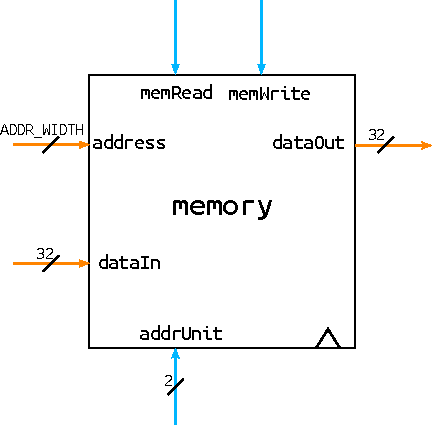
\includegraphics[scale=1]{../memory/ref/schematic/memory.pdf}
    \caption{Memory}
    \label{fig:memory}
\end{figure}

Figure \ref{fig:memory_timing} shows the usual timing diagram of this fully synchronous memory, according to which both reads and writes take place at the next clock cycle after the proper control signals are asserted.

\begin{figure}[hbtp]
    \centering
    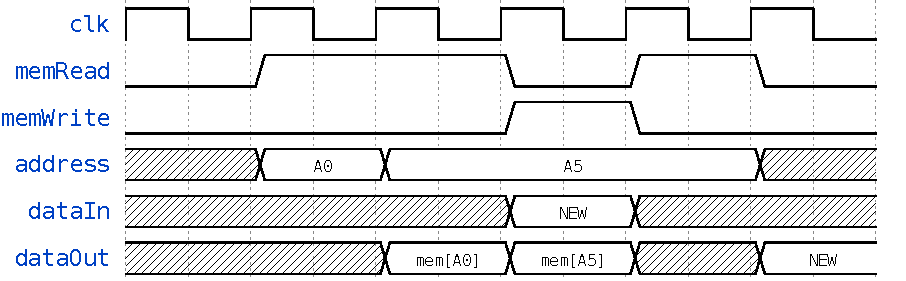
\includegraphics[scale=.8]{../memory/ref/timing/memory_timing.pdf}
    \caption{Memory timing diagram}
    \label{fig:memory_timing}
\end{figure}

\subsection{Register file}
The RISC-V register file is composed of 32 registers, each 32-bit wide (for RV32I), called \texttt{x0} to \texttt{x31}.

\subsection{ALU}



\end{document}